\documentclass[a4paper,twoside]{article}
\usepackage{cmap}
\usepackage{epsfig}
\usepackage{graphicx}
\usepackage{subcaption}
\usepackage{calc}
\usepackage{amssymb,amstext,amsmath,amsthm}
\usepackage{multicol}
\usepackage{pslatex}
\usepackage{apalike}
\usepackage{algorithm2e}
\usepackage[bottom]{footmisc}
\usepackage{booktabs}
\usepackage{array}
\usepackage{url}
\usepackage{SCITEPRESS}
\graphicspath{{figures/}}
\newcommand{\SAZ}{\ensuremath{S A Z}}
\newcommand{\PAZ}{\ensuremath{P A Z}}
\newif\ifanonymous
\anonymoustrue
\begin{document}
\title{Encoding Pen Dynamics in Handwriting Images: An Incremental Study of Parkinson's Disease Classification}
\ifanonymous
\author{\authorname{Anonymous Authors}\affiliation{Anonymous Institution}}
\else
\author{\authorname{Munif Gebara Jr.\sup{1}, \'Angel S\'anchez Calle\sup{2} and Yandre Maldonado e Gomes da Costa\sup{1}}
\affiliation{\sup{1}Departamento de Inform\'atica, Universidade Estadual de Maring\'a, Brazil}
\affiliation{\sup{2}Universidad Rey Juan Carlos, Spain}}
\fi
\keywords{Handwriting, Pseudodynamic Images, Local Phase Quantization, Parkinson's Disease, Explainable AI.}
\abstract{We introduce a new formulation of pseudodynamic handwriting minimap signatures that maps normalized pen signals onto contact-only trajectories. Using 597 PaHaW recordings from 75 participants, we progress from static traces to isolated colour signals and RGB combinations, then examine texture descriptors, learned features and task fusion. An initial eight-task comparison identifies task-dependent gains for speed, altitude and azimuth. A subsequent evaluation selects encodings and classifier parameters entirely within training, while spatial controls test the association between signals and trace positions. Neither analysis establishes an overall dynamic advantage after multiplicity correction. On three tasks fixed from prior work, training-selected encoding with Local Phase Quantization and SVM reaches participant-level macro F1 of 0.6449, compared with 0.6143 for static images, 0.6279 for kinematic/pressure features and 0.6021 for frozen ResNet18 transfer features. The numerical advantage remains uncertain. Reducing eight tasks to three helps some pipelines but not others. Grad-CAM analysis of the earlier scratch-trained CNN concentrates on writing but agrees poorly with occlusion. The study contributes an explicit encoding technique and a controlled account of how its performance depends on task selection, retained signal information and the learning procedure.}
\onecolumn\maketitle\normalsize\setcounter{footnote}{0}\vfill
\section{\uppercase{Introduction}}
\label{sec:introduction}
\begin{figure*}[t]
\centering
\resizebox{\textwidth}{!}{%
\begin{tikzpicture}[
  font=\footnotesize,
  stage/.style={draw=black!40, rounded corners=2pt, fill=#1, align=left, inner sep=4pt, minimum height=3.1cm, anchor=north west},
  exper/.style={draw=black!40, rounded corners=2pt, fill=#1, align=left, inner sep=4pt, text width=5.35cm, minimum height=2.55cm, anchor=north west},
  arr/.style={-{Stealth[length=2mm]}, thick, black!55},
]
\coordinate (bus) at (0,-3.5);
\coordinate (row2) at (0,-3.9);

\node[stage=blue!4, text width=3.6cm] (data) at (0,0)
  {\textbf{PaHaW recordings}\\[2pt]
   75 participants, 8 tasks,\\597 recordings\\[3pt]
   per sample: position, time, pen contact, pressure, altitude and azimuth};

\node[stage=orange!7, text width=4.0cm, right=5mm of data.north east, anchor=north west] (render)
  {\textbf{Pseudodynamic minimap}\\[2pt]
   \textbullet\ trace drawn only where the pen touches the tablet\\
   \textbullet\ each signal normalized within its own recording\\
   \textbullet\ azimuth centered on its circular mean\\
   \textbullet\ up to three signals mapped to RGB};

\node[stage=orange!7, text width=3.9cm, right=5mm of render.north east, anchor=north west] (enc)
  {\textbf{Nine encodings} (Table~\ref{tab:encoding})\\[3pt]
   \begin{tabular}{@{}c@{\hspace{8pt}}c@{}}
   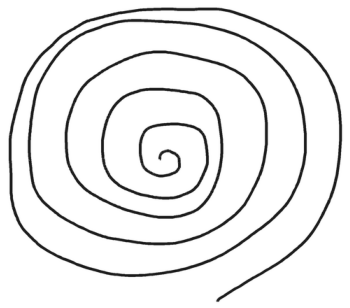
\includegraphics[height=1.2cm]{method_static.png} & 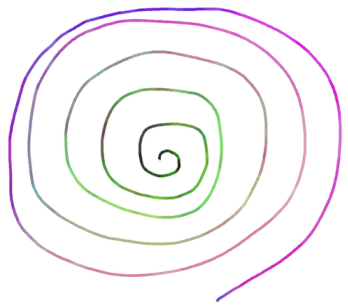
\includegraphics[height=1.2cm]{method_saz.png}\\
   \scriptsize 1: static trace & \scriptsize 8: $SAZ$
   \end{tabular}\\[2pt]
   2--5: one signal; 6--9: RGB triplets};

\node[stage=blue!4, text width=3.7cm, right=5mm of enc.north east, anchor=north west] (eval)
  {\textbf{Evaluation}\\[2pt]
   $5\times5$ participant-separated cross-validation with 3 inner folds\\[3pt]
   recording-level macro F1\\[1pt]
   participant-level macro F1 (majority vote over tasks)};

\node[exper=green!6] (e1) at (data.north west |- row2)
  {\textbf{Experiment 1} \hfill Sec.~\ref{sec:descriptor}--\ref{sec:classifiers}\\[2pt]
   all eight tasks\\[2pt]
   \textbullet\ each encoding described by LPQ texture and classified by SVM\\
   \textbullet\ leading encoding ($SAZ$): SVM compared with logistic regression, random forest and a CNN trained from scratch};

\node[exper=green!6, right=5mm of e1.north east, anchor=north west] (e2)
  {\textbf{Experiment 2} \hfill Sec.~\ref{sec:nested-followup}--\ref{sec:controls}\\[2pt]
   all eight tasks\\[2pt]
   \textbullet\ encoding, SVM and fusion rule chosen with training participants only\\
   \textbullet\ spatial controls: signals circularly shifted or permuted within each stroke};

\node[exper=green!6, right=5mm of e2.north east, anchor=north west] (e3)
  {\textbf{Experiment 3} \hfill Sec.~\ref{sec:competitive}\\[2pt]
   tasks T2--T4 (all eight as secondary)\\[2pt]
   \textbullet\ static trace + LPQ + SVM\\
   \textbullet\ minimaps + LPQ + SVM\\
   \textbullet\ minimaps + ResNet18 features\\
   \textbullet\ kinematic/pressure attributes + SVM};

\draw[arr] ([yshift=-1.55cm]data.north east) -- ([yshift=-1.55cm]render.north west);
\draw[arr] ([yshift=-1.55cm]render.north east) -- ([yshift=-1.55cm]enc.north west);
\draw[arr] ([yshift=-1.55cm]enc.north east) -- ([yshift=-1.55cm]eval.north west);

\draw[thick, black!55] (eval.south) -- (eval.south |- bus);
\draw[thick, black!55] (e1.north |- bus) -- (eval.south |- bus);
\foreach \e in {e1,e2,e3} \draw[arr] (\e.north |- bus) -- (\e.north);

\draw[arr, dashed, black!45] (data.north) -- ++(0,0.45)
  -| ([xshift=5mm,yshift=-2.05cm]e3.north east)
  node[pos=0.25, above, font=\scriptsize, text=black!70] {pen signals used directly, without an image}
  -- ([yshift=-2.05cm]e3.north east);
\end{tikzpicture}}
\caption{Overview of the method. Each PaHaW recording is rendered as a pseudodynamic minimap in one of nine encodings, and every experiment uses the same participant-separated cross-validation. Experiment~1 compares encodings and classifiers, Experiment~2 chooses the encoding with training participants only and tests whether the position of the signals along the stroke matters, and Experiment~3 compares minimaps with the static trace and with kinematic/pressure attributes computed directly from the pen signals (dashed arrow). Thumbnails show the spiral of one healthy participant as rendered.}
\label{fig:method}
\end{figure*}

\noindent
A digitizing tablet records the pen trajectory together with its speed, pressure and inclination. Encoding these measurements as colour adds information about how a trace was produced while keeping its recognizable shape, so that standard image descriptors and classifiers can use the dynamics directly.

The application is the distinction between Parkinson's disease (PD) and healthy participants (H) in PaHaW, a database of online handwriting and drawing tasks \cite{Drotar2016}. Handwriting exposes aspects of fine motor behaviour, and the relation between pen motion and diagnosis depends on the task, device and participant characteristics \cite{Impedovo2019}.

We propose \emph{pseudodynamic minimaps}, a new image representation of a handwriting task execution. Planar position supplies the image coordinates and colour carries the measured pen attributes. The term minimap follows work that renders source code compactly as a visual signature \cite{Gebara2025}.

Handwriting classification has often used explicitly designed kinematic and pressure features, as in the study that introduced PaHaW \cite{Drotar2016}. Learned features provide another route, either from pen dynamics \cite{Pereira2016} or from visual attributes of reconstructed writing \cite{Moetesum2019}. Dynamic information has also appeared in earlier handwriting images: Diaz et al. encode movement through acquired points and pen-up trajectories for PD detection \cite{Diaz2019}, and Cilia et al. build synthetic RGB images from handwriting dynamics for Alzheimer's disease detection \cite{Cilia2021SyntheticImages}.

Rendering a temporal signal as an image is an established route to reusing visual descriptors and convolutional models. Recurrence plots expose the recurrence structure of a dynamical system as a two-dimensional pattern \cite{Eckmann1987}, Gramian angular fields and Markov transition fields encode a univariate series as a matrix \cite{Wang2015}, and convolutional networks trained on such renderings are competitive on time-series benchmarks \cite{Hatami2018}. The same reduction appears outside the time domain, where source code is rendered as an image for classification \cite{Shi2022}.

Pseudodynamic minimaps differ from these transforms in three respects. The image coordinates are the physical positions the pen visited rather than a time axis, so each signal value stays anchored to the stroke that produced it. Each signal is normalized within its own recording by percentiles, so colour describes the writer's relative variation. Azimuth is centred on its circular mean, so that the arbitrary zero-degree boundary does not separate similar orientations.

This initial study evaluates the representation in three experiments that share participant-separated partitions (Figure~\ref{fig:method}). Experiment~1 adds speed, pressure, altitude and azimuth to the static trace, one at a time and as RGB triplets, and compares classifiers on the leading encoding. Experiment~2 selects the encoding with training participants only and displaces the signals along each stroke to test whether their position matters. Experiment~3 compares minimaps, described by LPQ texture or by pretrained ResNet18 features, with the static trace and with kinematic/pressure attributes on the repeated \textit{l}, \textit{le} and \textit{les} tasks examined in earlier work on PaHaW \cite{Casademunt2023}.

The results indicate that the classifiers make use of the encoded dynamics. Training-only selection preferred a dynamic encoding over the static trace in almost every training set, displacing the signals along the stroke lowered performance, and on the three repeated-pattern tasks the minimap pipeline gave the best observed participant-level decisions among the four pipelines. A cohort of 75 participants leaves the size of these gains uncertain; the study establishes how pen dynamics can be carried into an image and where they help, rather than delivering a clinical tool.

\section{\uppercase{Building the Minimap Representation}}
\label{sec:encoding}

\noindent
To vary the information encoded in each minimap, we first reconstruct the visible trace. We then map individual pen signals to color and combine them without changing the trajectory or rendering geometry.

\subsection{The Visible Trace}
\noindent
Let $q_i$, $i=1,\dots,N$, be the samples or points of a handwriting task recording:
\begin{equation}
 q_i=(x_i,y_i,t_i,s_i,z_i,a_i,p_i),
\end{equation}
where $x_i$ and $y_i$ are the spatial coordinates of sample $i$, $t_i$ is its timestamp, $s_i$ indicates surface contact (i.e., ``on-surface'' or ``in-air''), $z_i$ is the azimuth, $a_i$ represents the altitude and $p_i$ is the pen pressure. The stored PaHaW columns place $y$ before $x$ coordinates; the renderer restores their planar order. Image rows follow the tablet's vertical coordinate without inversion, so every minimap is a vertically mirrored view of the writing; the transformation is identical for all records and both classes, and Figures~\ref{fig:tasks} and~\ref{fig:controls-examples} show the writing in its natural orientation.

The static image uses only position and the contact indicator. A segment between samples $i$ and $i+1$ is drawn if both samples are on the surface:
\begin{equation}
 \mathcal{S}=\{i:s_i=1\ \mathrm{and}\ s_{i+1}=1\}.
\end{equation}
This preserves pen lifts as gaps instead of joining the end of one stroke to the beginning of the next. Neither the in-air trajectory nor the duration of a lift appears in the image. Contact points alone determine its bounding box, which is centered on a $512\times512$ white canvas with a 20-pixel margin, using one scale factor for both axes. Segments are drawn in RGB $(30,30,30)$ with constant 4-pixel thickness. Rendering takes place at three times the target resolution and is reduced with Lanczos filtering. These settings remain fixed throughout the color experiments.

The image retains form and stroke discontinuities, but fitting every record to its own canvas removes absolute size. Geometrically similar samples of different sizes can produce the same image, discarding the absolute size information relevant to micrographia.

\subsection{Adding One Signal}
\begin{figure*}[t]
\centering
\setlength{\unitlength}{\textwidth}
\begin{picture}(1,0.444)
\put(0.025,0){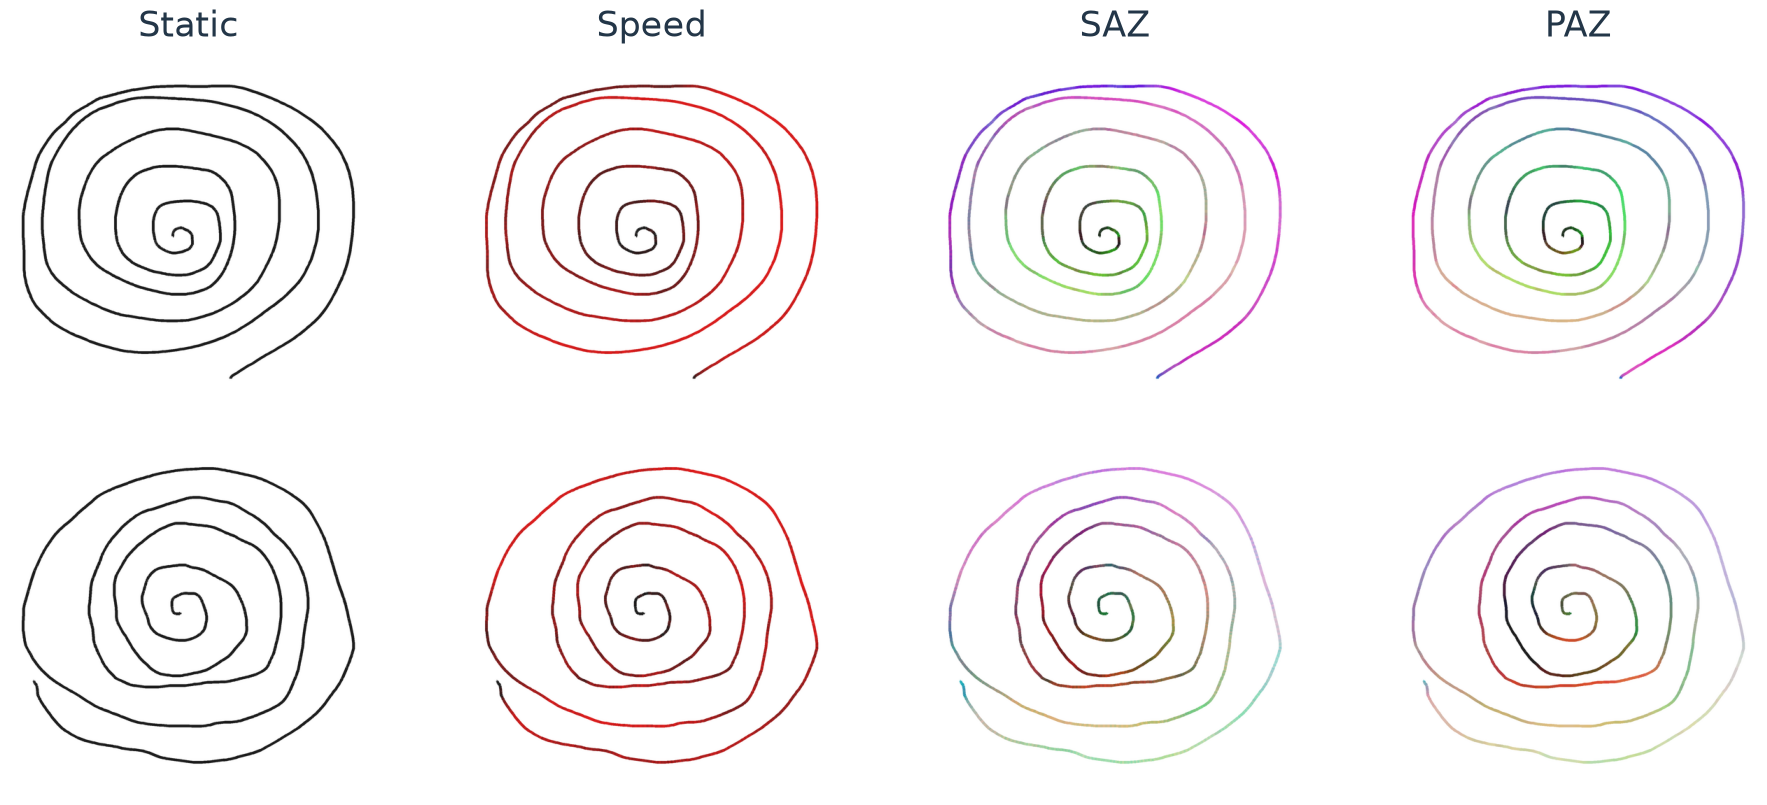
\includegraphics[width=0.975\textwidth]{progressive_encoding_nolabels.png}}
\put(0.010,0.322){\makebox(0,0){\rotatebox{90}{\small Healthy example}}}
\put(0.010,0.105){\makebox(0,0){\rotatebox{90}{\small PD example}}}
\end{picture}
\caption{Building a pseudodynamic minimap from the same spiral trace. Rows show one healthy and one PD example, selected by a fixed identifier rule without reference to prediction quality. Columns move from the static trace (encoding~1 in Table~\ref{tab:encoding}) to speed alone (2) and two RGB triplets, $SAZ$ (8) and $PAZ$ (9). The trajectory is unchanged; color describes within-recording variation.}
\label{fig:progressive}
\end{figure*}
\noindent
Four measurements are candidates for color: speed ($S$), pressure ($P$), altitude ($A$) and azimuth ($Z$). Altitude describes pen inclination relative to the surface, while azimuth describes its orientation in the tablet plane. We first encode each signal alone (encodings 2--5 in Table~\ref{tab:encoding}), always in the red channel, with green and blue fixed at 30. This avoids changing the channel assignment while screening the signals.

For a surface segment, speed is calculated directly from the consecutive coordinates and timestamps:
\begin{equation}
 v_i=\frac{\sqrt{(x_{i+1}-x_i)^2+(y_{i+1}-y_i)^2}}{t_{i+1}-t_i}.
 \label{eq:speed}
\end{equation}
We use $\log(1+v_i)$ in the tablet's native coordinate and time units. This compresses large values before the intensity mapping. Pressure and altitude use the arithmetic mean of the two endpoint measurements.

Azimuth requires a circular reference. We convert the recorded tenths of a degree to radians and compute the mean direction over contact samples. Each angle is centered on that direction and wrapped into $[-\pi,\pi]$ before the endpoint average is taken. This reduces the effect of an arbitrary zero-degree boundary. It is a circular centering operation, not temporal unwrapping, and it does not remove every possible branch-cut artifact.

Each transformed signal is scaled within the recording being rendered. Let $q_{.05}$ and $q_{.95}$ be its fifth and ninety-fifth percentiles over surface segments. The normalized value is
\begin{equation}
 u_i=\operatorname{clip}\left(\frac{f_i-q_{.05}}{q_{.95}-q_{.05}},0,1\right),
 \label{eq:normalization}
\end{equation}
with $u_i=0.5$ if the percentile range is degenerate. We map it to an integer channel value
\begin{equation}
 c_i=\operatorname{round}(30+190u_i).
 \label{eq:color}
\end{equation}
The white background stays outside the semantic range. Anti-aliasing introduces intermediate intensities at boundaries, as in the static reconstruction.

Each record is normalized independently, without a cohort-wide reference distribution or class labels. Color therefore describes relative variation within a recording: the same red value in two images need not represent the same absolute speed or pressure. Circular centering also removes absolute pen orientation. These quantities remain available to methods that use the physical measurements directly.

\subsection{Combining Signals in RGB}
\noindent
We assign one scalar signal to each RGB channel and evaluate all four subsets of size three (encodings 6--9). Table~\ref{tab:encoding} numbers the nine encodings used throughout the paper, and Figure~\ref{fig:progressive} illustrates the progression. All combinations use the same geometry, background and rendering settings as the static and single-signal images.

\begin{figure*}[t]
\centering
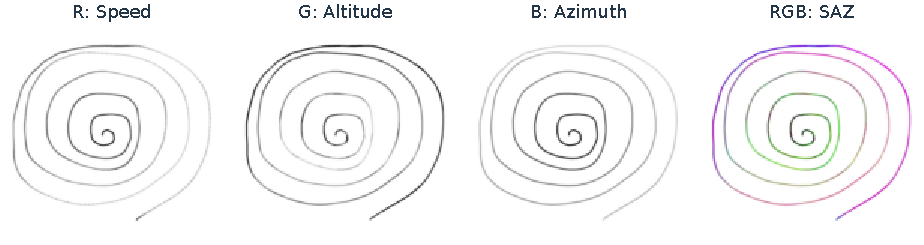
\includegraphics[width=0.9\textwidth]{rgb_semantics.pdf}
\caption{The three channels of an $SAZ$ minimap (encoding~8), shown individually in grayscale and combined as RGB. Darker gray marks a lower channel value. Red stores log-speed, green altitude and blue circularly centered azimuth, each normalized within the recording.}
\label{fig:rgb}
\end{figure*}

Figure~\ref{fig:rgb} decomposes an $SAZ$ minimap into its channels. In this spiral, speed is lowest near the center and rises along the outer turns, while altitude and azimuth vary over different portions of the trajectory; the RGB image places all three variations on the same stroke.

\begin{table}[t]
\centering\small
\caption{The nine encodings, numbered as used throughout the paper. A dash denotes a constant channel value of 30. $S$: speed; $P$: pressure; $A$: altitude; $Z$: azimuth.}
\label{tab:encoding}
\begin{tabular}{clccc}
\toprule
\# & Encoding & Red & Green & Blue\\
\midrule
1 & Static & -- & -- & --\\
\midrule
2 & $S$ & $S$ & -- & --\\
3 & $P$ & $P$ & -- & --\\
4 & $A$ & $A$ & -- & --\\
5 & $Z$ & $Z$ & -- & --\\
\midrule
6 & $SPA$ & $S$ & $P$ & $A$\\
7 & $SPZ$ & $S$ & $P$ & $Z$\\
8 & $SAZ$ & $S$ & $A$ & $Z$\\
9 & $PAZ$ & $P$ & $A$ & $Z$\\
\bottomrule
\end{tabular}
\end{table}

Because the descriptor applies the same histogram construction to each channel, permuting the RGB assignment only permutes three feature blocks, and standardization followed by a linear or radial-basis SVM is invariant to that permutation apart from numerical effects. Each triplet therefore needs one assignment rather than six for the SVM experiment. The argument does not extend to every image model, and the CNN receives one fixed assignment.

Segments are drawn in acquisition order. A later segment can overwrite an earlier color at a crossing, and the image has no separate layer for repeated visits to the same position. It preserves spatially located signal variation, not the complete sample sequence. Calling the result pseudodynamic reflects that distinction.

\section{\uppercase{Data and Evaluation}}
\label{sec:protocol}

\noindent
The evaluation is organized as three experiments that share the same participant partitions. Experiment~1 (Sections~\ref{sec:descriptor}--\ref{sec:classifiers}) compares the nine encodings of Table~\ref{tab:encoding} under a fixed descriptor and classifier. Experiment~2 (Sections~\ref{sec:nested-followup} and~\ref{sec:controls}) selects the encoding using training participants only and tests controls that displace the signals along each stroke. Experiment~3 (Section~\ref{sec:competitive}) compares minimaps, described by LPQ texture or by pretrained ResNet18 features, with the static trace and with kinematic/pressure attributes on three tasks fixed from prior work.

\subsection{The PaHaW Dataset}
\label{sec:dataset}
\noindent
PaHaW was acquired with the First Department of Neurology at St.Anne's University Hospital in Brno and includes 37 PD patients (19 men) and 38 healthy participants (20 men) \cite{Drotar2016}. All participants were native Czech speakers who wrote with their dominant right hand, and the patients were recorded under L-DOPA medication. They wrote with an inking pen on an empty paper template laid over a Wacom Intuos 4M tablet, which gave normal visual feedback, while a predefined template showed each task; neither the number of repetitions nor the writing height was imposed. The tablet sampled the pen at 100 samples per second during on-surface and in-air movement, recording position, pressure and pen status, and the released recordings also contain altitude and azimuth. The dataset has since been used to study which handwritten elements carry Parkinsonian alterations \cite{Casademunt2024}.

\begin{figure}[t]
\centering\footnotesize
\setlength{\tabcolsep}{2pt}
\begin{tabular}{@{}cc@{}}
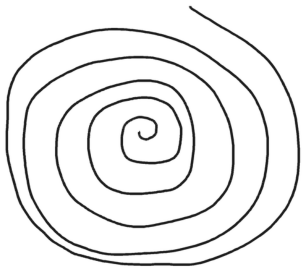
\includegraphics[width=0.47\columnwidth]{tasks/T1.png} & 
\includegraphics[width=0.47\columnwidth]{tasks/T2.png}\\
T1 Spiral & T2 \textit{l}\\[3pt]

\includegraphics[width=0.47\columnwidth]{tasks/T3.png} & 
\includegraphics[width=0.47\columnwidth]{tasks/T4.png}\\
T3 \textit{le} & T4 \textit{les}\\[3pt]

\includegraphics[width=0.47\columnwidth]{tasks/T5.png} & 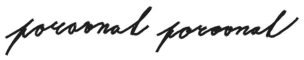
\includegraphics[width=0.47\columnwidth]{tasks/T6.png}\\
T5 \textit{lektorka} & T6 \textit{porovnat}\\[3pt]
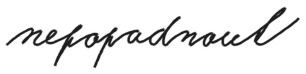
\includegraphics[width=0.47\columnwidth]{tasks/T7.png} & 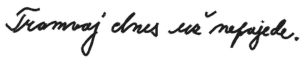
\includegraphics[width=0.47\columnwidth]{tasks/T8.png}\\
T7 \textit{nepopadnout} & T8 Sentence\\
\end{tabular}
\caption{The eight PaHaW tasks written by one healthy participant, shown as static traces in writing orientation. Each recording is scaled separately, so absolute writing size is not preserved.}
\label{fig:tasks}
\end{figure}

The eight tasks progress from drawing to writing (Table~\ref{tab:tasks} and Figure~\ref{fig:tasks}). T1 is an Archimedean spiral drawn from the inside out. T2--T4 repeat the cursive letter \textit{l}, the bigram \textit{le} and the trigram \textit{les}. T5--T7 repeat the Czech words \textit{lektorka}, \textit{porovnat} and \textit{nepopadnout}, which can be written without lifting the pen, and T8 is the sentence \textit{Tramvaj dnes u\v{z} nepojede}, which adds in-air transitions between words \cite{Drotar2016}. Our local copy contains 597 recordings from the 75 participants: three spiral recordings are absent, and every other task has one recording per participant. We retain all available records and do not interpret missing files as quality exclusions.

\begin{table}[t]
\centering\small
\caption{Task inventory. T1 contains 36 PD and 36 H records; each other task contains 37 PD and 38 H records.}
\label{tab:tasks}
\begin{tabular}{clr}
\toprule
ID & Task & Records\\
\midrule
T1 & Archimedean spiral & 72\\
T2 & Repeated \textit{l} & 75\\
T3 & Repeated \textit{le} & 75\\
T4 & Repeated \textit{les} & 75\\
T5 & Repeated \textit{lektorka} & 75\\
T6 & Repeated \textit{porovnat} & 75\\
T7 & Repeated \textit{nepopadnout} & 75\\
T8 & \textit{Tramvaj dnes u\v{z} nepojede.} & 75\\
\bottomrule
\end{tabular}
\end{table}

An input audit checked file counts, sample counts, finite values and timestamp increments. Five files declare a sample count different from the rows present, and the renderer uses the rows available. We calculate speed from the recorded timestamps rather than an assumed sampling interval. Of the 253 negative timestamp increments, none falls inside a contact segment: all 1,065,788 segments with contact at both endpoints increase in time, so Equation~\ref{eq:speed} requires no interpolation. No normalization range was degenerate.

The participant is the independent observational unit; tasks and alternative renderings do not enlarge the cohort. Mean age is 69.32 years in PD and 62.42 in H. Age and clinical fields are excluded from classifier inputs, but handwriting may still reflect this difference.

\subsection{A Common Partition for Every Task}
\noindent
We construct stratified folds from one row per participant, then propagate the assignments to every task and rendering. Five repetitions of five outer folds produce a test prediction for every available record in each repetition, and all tasks from a participant fall in the same outer fold.

Within each outer training partition, three participant-separated inner folds choose the model hyperparameters. Feature standardization is fitted on the corresponding training portion, never on its validation or test participants. The selected model is refitted on all outer training participants and evaluated once on the outer test set. Rendering is independent per record, so it learns nothing from other records before splitting.

In Experiment~1, each fixed encoding and classifier yields 200 outer models and 2,985 outer-test predictions, which are repeated predictions of 597 records from 75 participants. Experiment~1 chooses its leading encoding from these outer-test scores for the classifier comparison, so Experiments~2 and~3 repeat the encoding choice with training participants only, using three inner folds common across tasks.

\subsection{Metrics and Statistical Analysis}
\noindent
Macro F1 gives equal weight to the two diagnosis classes:
\begin{equation}
 F_{\mathrm{macro}}=\frac{F_{1,\mathrm{H}}+F_{1,\mathrm{PD}}}{2}.
\end{equation}
Each recording receives its own prediction. For each task and repetition we pool the five outer-test folds and compute this \emph{recording-level} macro F1 once, then average the five repetitions. Averaging over the eight tasks gives the recording-level endpoint used to rank encodings,
\begin{equation}
 \overline F_{\mathrm{rec}}=\frac{1}{8\cdot5}\sum_{t=1}^{8}\sum_{r=1}^{5}F_{t,r},
 \label{eq:taskmetric}
\end{equation}
and Experiment~3 uses the corresponding mean over T2--T4. The \emph{participant-level} endpoint combines the tasks into one decision per participant (Section~\ref{sec:fusion}). We also report accuracy, balanced accuracy, PD sensitivity, H specificity and ROC AUC.

We calculate 95\% percentile confidence intervals from 10,000 diagnosis-stratified bootstrap draws of participants; each draw keeps all of a participant's tasks and repeated predictions, and a paired contrast applies the same draw to both methods. The randomization test exchanges method predictions per participant, jointly across tasks and repetitions, using 10,000 swap patterns. Both procedures keep the fitted models fixed, so they describe uncertainty in these predictions without the variability of retraining.

Holm adjustment is applied within declared families. In Experiment~1 these are the 36 encoding pairs, the per-task contrasts of single signals and of triplets against static (32 each), the six classifier pairs at each endpoint, the three fusion-rule pairs and eight per-task CNN--SVM contrasts; Experiments~2 and~3 declare their own families. With 75 participants, the advantage of the LPQ models over the scratch-trained CNN (Section~\ref{sec:classifiers}) is the difference that survives its family. We therefore report effect sizes with their 95\% intervals throughout and give adjusted $p$ values where they are informative.

\subsection{One Decision per Participant}
\label{sec:fusion}
\noindent
Each task model predicts every held-out participant, and three rules combine these predictions into one decision per participant. \emph{Probability averaging} takes the mean of the calibrated PD probabilities across tasks. \emph{Weighted averaging} does the same but gives more weight to tasks whose models scored higher on validation participants drawn from the training set. \emph{Majority voting} assigns the class predicted by most tasks, with ties assigned to PD. A missing spiral recording is left out of that participant's decision, and because every task shares the participant folds, no model contributing to a participant's decision was trained on that participant. The metric is computed for each repetition and averaged over the five. In Experiment~1 the three rules gave similar macro F1 (0.6341, 0.6447 and 0.6488); Experiment~2 chooses the rule within training, and Experiment~3 fixes majority voting before fitting.

\section{\uppercase{Encoding the Dynamics}}
\label{sec:representation-results}

\noindent
Experiments~1 and~2 compare the encodings on common participant partitions. LPQ extraction and SVM selection are held fixed, so that each comparison changes only the image encoding.

\subsection{A Fixed Descriptor for the Comparison}
\label{sec:descriptor}
\noindent
Local Phase Quantization describes texture through local Fourier phase information \cite{Ojansivu2008}. We apply the same implementation independently to each RGB channel.

The choice of LPQ was motivated by its encoding of local phase relationships in compact histograms, which tolerates blur \cite{Ojansivu2008} and is therefore less sensitive to the smoothing introduced by resizing, rasterization and anti-aliasing. This property suits pseudodynamic minimaps drawn with a fixed line width, where the relevant information lies in the spatial organization of the strokes and in local variations of the semantic RGB channels (speed, pressure, altitude and azimuth) rather than in stroke thickness. The selection was informed by preliminary comparisons with other texture and shape descriptors, namely grayscale and semantic RGB Local Binary Patterns (LBP), opponent LBP, GLCM/Haralick statistics, Gabor filters, Histograms of Oriented Gradients (HOG) and wavelet-based features. No alternative was consistently superior across tasks, and LPQ offered a favorable balance between compactness, robustness and sensitivity to the fine local patterns encoded in the minimaps.

Before extraction, foreground is detected by any channel intensity below 250. We crop its bounding box, add a margin equal to 5\% of the longer dimension, pad to a square with white, and resize to $64\times64$ by bilinear interpolation. LPQ filters each channel with four complex $5\times5$ kernels at frequency offsets $(1,0)$, $(0,1)$, $(1,1)$ and $(1,-1)$, scaled by $1/5$. The signs of their real and imaginary responses form an eight-bit code at each pixel, using reflected boundaries. We normalize a 256-bin histogram by its count, take its element-wise square root, and concatenate the channels. The 768-attribute vector includes the padded background. No decorrelation or spatial pyramid is applied.

The static RGB channels are identical, so the static vector repeats the same histogram three times. This keeps the interface and nominal dimension constant; it does not create additional static information. For the single-signal encodings, two channels remain constant along the trace and retain its geometric pattern.

Standardization and support vector machine fitting \cite{Cortes1995} occur inside each training partition. The search contains five linear models with $C\in\{0.01,0.1,1,10,100\}$ and sixteen radial-basis models with $C\in\{0.1,1,10,100\}$ and $\gamma\in\{\mathrm{scale},10^{-4},10^{-3},10^{-2}\}$. We use inverse-frequency class weights. The candidate with the highest mean inner-fold macro F1 is chosen, with ties resolved by the stored candidate order. The SVM learns from LPQ image texture and receives no original signal measurements as tabular features.

\subsection{The Static Baseline}
\label{sec:static-baseline}
\noindent
Experiment~1 starts from the static trace (encoding~1), which reaches a recording-level macro F1 of 0.5643 over the eight tasks. Its best task is repeated \textit{les} (T4), with 0.6502 and a participant-bootstrap interval of [0.5582, 0.7351]; the spiral reaches 0.5915 and T5 0.5038.

\subsection{Single Signals and RGB Combinations}
\begin{figure*}[t]
\centering
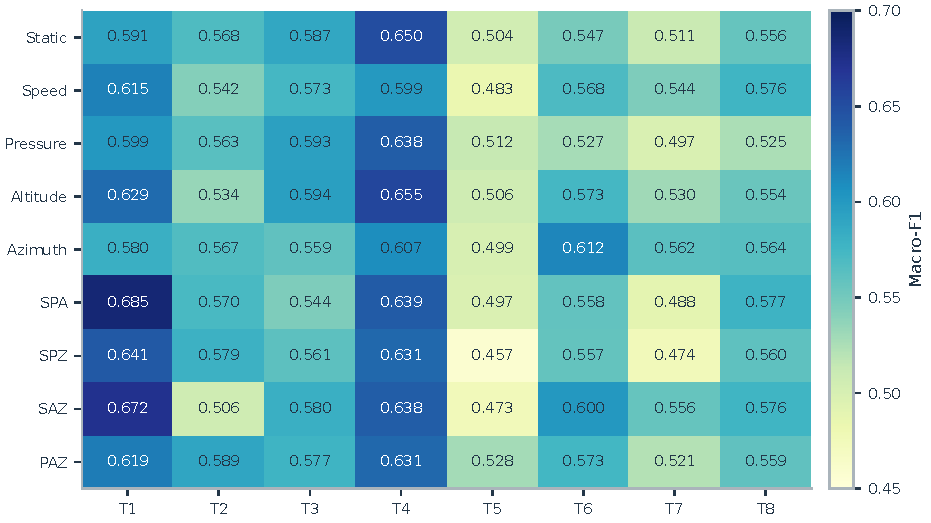
\includegraphics[width=0.8\textwidth]{encoding_heatmap.pdf}
\caption{Recording-level macro F1 of Experiment~1 for every encoding and task, averaged over five repetitions. Rows follow Table~\ref{tab:encoding}, from the static trace (1) to $PAZ$ (9). Color helps most on the spiral (T1), and the best encoding differs between tasks.}
\label{fig:heatmap}
\end{figure*}
\noindent
Altitude and azimuth are the most informative single signals. Altitude (encoding~4) reaches a recording-level macro F1 of 0.5718 and azimuth (5) 0.5688, both above the static trace, while speed (2) reaches 0.5625 and pressure (3) 0.5568. The gains concentrate on specific tasks: altitude raises the spiral from 0.5915 to 0.6294 while keeping T4 at 0.6548, and speed raises the spiral to 0.6153 but lowers T4 from 0.6502 to 0.5994.

Figure~\ref{fig:heatmap} shows where the dynamics help. Every encoding except azimuth alone raises the spiral above the static trace, and the RGB triplets give its highest scores: $SPA$ (6) reaches 0.685 and $SAZ$ (8) 0.672, against 0.591. Azimuth lifts T6 from 0.547 to 0.612, altitude gives the best T4, and T5 remains difficult for every encoding.

Combining three signals gives the best encodings of Experiment~1. $SAZ$ (8) reaches 0.5752, followed by $PAZ$ (9) at 0.5746, $SPA$ (6) at 0.5697 and $SPZ$ (7) at 0.5574. $SAZ$ improves the spiral by 0.0802, T6 by 0.0524 and T7 by 0.0455, and lowers T2 by 0.0612; its paired gain over the static trace is +0.0109 [$-$0.0146, 0.0370]. The near tie between $SAZ$ and $PAZ$ suggests that speed and pressure are largely interchangeable alongside the two pen angles. Because $SAZ$ was chosen as the leading encoding from outer-test scores, Experiment~2 repeats the choice with training participants only.

\subsection{Classifier and Fusion Choices}
\label{sec:classifiers}
\noindent
Holding $SAZ$ and the participant partitions fixed, Experiment~1 also varies the classifier on the same 768 LPQ attributes. SVM leads with a recording-level macro F1 of 0.5752, ahead of regularized logistic regression at 0.5674 and a Random Forest of 100 trees at 0.5599 \cite{Breiman2001}, with Holm-adjusted $p=0.6563$ and $p=0.5645$ for the two gaps. A compact convolutional network trained from scratch on $128\times128$ pixels, in the tradition of convolutional models for document recognition \cite{LeCun1998}, reaches 0.5105. All three LPQ models outperform it, and these differences survive correction: the SVM margin is 0.0646 [0.0277, 0.1021] at adjusted $p=0.0054$, and logistic regression and Random Forest reach adjusted $p=0.0255$ and $p=0.0460$. The comparison also reflects differences in input resolution and search budget, and pretrained CNN features behave differently in Experiment~3. After participant fusion, logistic regression reaches 0.6498 and SVM 0.6488. We carry the SVM forward as the reference classifier.

\subsection{Choosing the Encoding Within Training}
\label{sec:nested-followup}
\noindent
Experiment~2 evaluates the procedure that chooses an encoding. It keeps the outer participant partitions and adds three inner folds common across tasks. Within each outer training set, each task and encoding receives the same 21-candidate SVM search, and one encoding is chosen for all eight tasks by the unweighted mean of the selected per-task scores, with ties resolved in favor of the static trace. We compare a fixed static policy, selection among all nine encodings, and selection among the eight dynamic encodings.

Experiment~2 also chooses the fusion rule without the test participants. The training participants are split into three parts; on each split, encoding and SVM selection are repeated on two parts and the third is predicted. These validation predictions choose the rule, after which the encoding and per-task models are selected again on all training participants. Calibration uses training participants only, and every choice is saved before the test participants are scored.

Training data consistently favor the dynamics. Although ties went to the static trace, selection among all nine encodings chose a dynamic encoding in 24 of the 25 outer training sets. No single signal dominates: in the dynamic-only policy, azimuth (5) was chosen five times and $SAZ$ (8) four times. On the recording-level endpoint the dynamic-only policy reaches 0.5643 and the nine-encoding policy 0.5618, against 0.5620 for static, with paired differences of +0.0023 [$-$0.0172, 0.0221] and $-$0.0002 [$-$0.0192, 0.0190]. One encoding chosen for eight heterogeneous tasks averages gains with losses, from +0.0567 on the spiral to $-$0.0274 on T5 for the dynamic-only policy. With the fusion rule also chosen inside training, participant-level macro F1 is 0.6017 for dynamic-only and 0.5991 for nine-encoding selection, against 0.6171 for static. Experiment~3 therefore tests the selected encoding on a shorter and more homogeneous task set.

\subsection{Controls of the Signal--Position Association}
\label{sec:controls}
\noindent
Adding color changes both the signal content and the image texture. Two controls keep the ingredients of the texture and change only where each signal value occurs: a nonzero circular shift by 25--75\% of the segments within each pen-down stroke, and a joint permutation of the segments within that stroke. The three channels move together, so each segment keeps its combination of values; single-segment strokes are unchanged and no value crosses a pen lift. Both controls keep geometry, line width and normalization, and permutation additionally breaks the continuity of the signal along the stroke (Figure~\ref{fig:controls-examples}). Each control transforms training and test recordings with three fixed seeds and repeats the dynamic-only selection; metrics are averaged over seeds, and bootstrap draws keep each participant's tasks, repetitions and seeds together.

\begin{figure*}[t]
\centering
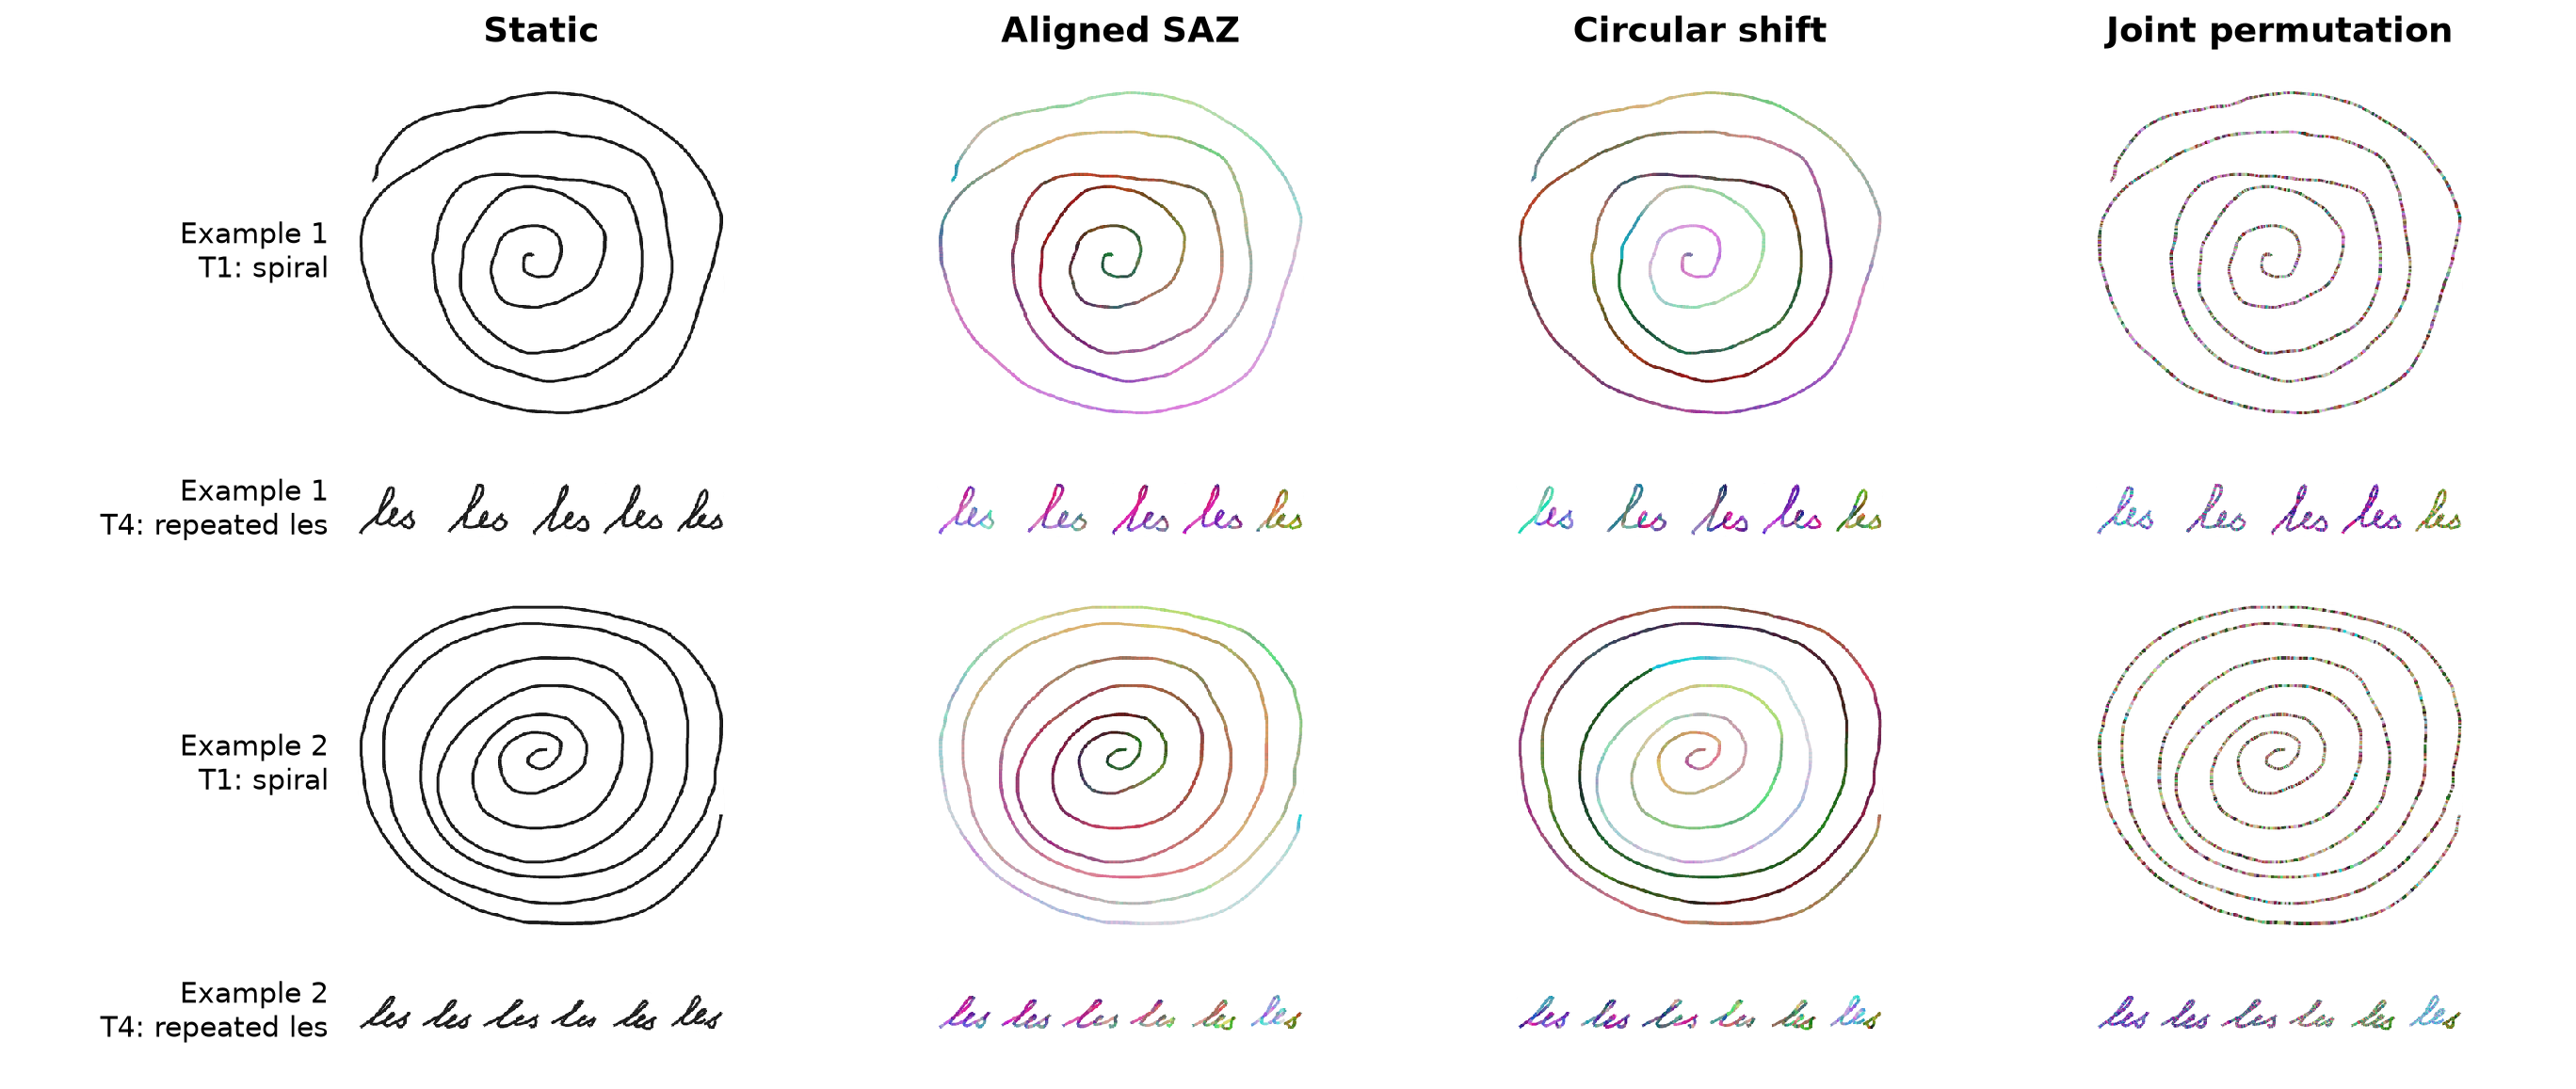
\includegraphics[width=\textwidth]{spatial_controls_cropped.png}
\caption{The two controls of Experiment~2 applied to the spiral (T1) and repeated \textit{les} (T4) of two participants, with seed 20260909. Aligned $SAZ$ is the unpermuted encoding. Geometry, pen-down segments and line width are unchanged; circular shifts move coherent runs of color along each stroke, whereas joint permutation scatters them. The rendered images are flipped vertically for display, so the writing appears in its natural orientation (Section~\ref{sec:encoding}); they were not selected by classifier performance.}
\label{fig:controls-examples}
\end{figure*}

\begin{table*}[t]
\centering\small
\caption{Experiment~2 on all eight tasks. Recording-level macro F1 with 95\% participant-bootstrap intervals. $\Delta$ is the difference from the static trace for the two selection policies, and dynamic-only selection minus the control for the two controls. Controls average three fixed seeds.}
\label{tab:nested-controls}
\begin{tabular}{@{}lll@{}}
\toprule
Policy & Macro F1 [95\% CI] & $\Delta$ [95\% CI]\\
\midrule
Static trace (fixed) & 0.5620 [0.5120, 0.6082] & --\\
Selection among nine encodings & 0.5618 [0.5122, 0.6082] & $-$0.0002 [$-$0.0192, 0.0190]\\
Selection among dynamic encodings & 0.5643 [0.5141, 0.6114] & +0.0023 [$-$0.0172, 0.0221]\\
Circular-shift control & 0.5561 [0.5093, 0.5990] & +0.0082 [$-$0.0102, 0.0264]\\
Joint-permutation control & 0.5442 [0.4956, 0.5885] & +0.0201 [0.0010, 0.0399]\\
\bottomrule
\end{tabular}
\end{table*}

Table~\ref{tab:nested-controls} summarizes Experiment~2. Displacing the signals within strokes lowered recording-level macro F1 from 0.5643 to 0.5561 under circular shifts and to 0.5442 under joint permutation, a decrease of 0.0201 [0.0010, 0.0399] whose interval lies above zero. The effect is largest on the spiral, where permutation removes 0.0609 [0.0086, 0.1174]. This pattern indicates that performance depends on where the dynamics are placed along the trajectory, not only on the colors present in the image. The four contrasts of this experiment, the two selection policies against static and dynamic-only selection against each control, form one Holm family, in which the permutation effect has adjusted $p=0.1848$; confirming it will require a larger cohort.

\subsection{Which Classifier and Fusion Rule}
\label{sec:classifiers}
\noindent
Holding $SAZ$ and the participant partitions fixed, an exploratory comparison on the same 768 LPQ attributes places SVM first at a task mean of 0.5752, ahead of regularized logistic regression at 0.5674 and a Random Forest of 100 trees at 0.5599 \cite{Breiman2001}; neither gap is supported, with Holm-adjusted $p=0.6563$ and $p=0.5645$ in a six-pair family. A compact convolutional network trained from scratch on $128\times128$ pixels \cite{LeCun1998} reaches 0.5105, below all three LPQ models: the SVM--CNN difference is 0.0646 [0.0277, 0.1021] with adjusted $p=0.0054$. That contrast confounds architecture with input resolution and search budget, and Section~\ref{sec:competitive} shows pretrained features behaving differently. After participant fusion the ranking flattens, with logistic regression at 0.6498 and SVM at 0.6488 and no supported pairwise difference. All of these estimates are conditional on having selected $SAZ$ from outer scores, so we carry the SVM forward as a fixed procedure rather than as a validated best classifier.

\section{\uppercase{Competitive Baselines}}
\label{sec:competitive}

\noindent
Experiment~3 compares the selected minimaps with methods that use the original movement signals and pretrained visual features. It uses a task set drawn from related work, which also shortens the handwriting protocol, and keeps all eight tasks as a secondary comparison.

\subsection{Task Set and Evaluation Protocol}
\noindent
The primary set comprises repeated \textit{l}, \textit{le} and \textit{les} (T2--T4), the tasks examined in the reference thesis~\cite{Casademunt2023}. We fix this set before fitting the models, and combining its three tasks by voting is our adaptation. Four methods are evaluated: static LPQ with SVM, LPQ with selection among the nine encodings, a kinematic/pressure SVM, and a frozen ResNet18 with a trained linear classification head.

The methods share the 25 outer participant partitions and three common inner folds. For each task and eligible encoding, mean inner-fold macro F1 selects the classifier parameters, and the two image methods that allow encoding selection choose one encoding for the task set by averaging these scores across its tasks, with ties resolved in favour of the static trace. Each method makes its own choices using only outer-training participants; standardization is fitted within the training partition, and selected models are refitted on the complete outer-training set. The three SVM methods retain the same 21-candidate linear/RBF search.

The primary endpoint is participant-level macro F1 from majority voting over T2--T4 (Section~\ref{sec:fusion}), with no calibration, learned weights or rule selection. Recording-level macro F1 over the three tasks is secondary. Holm adjustment covers the six method pairs separately at each endpoint, and the four within-method contrasts between three-task and eight-task voting form another family.

\subsection{Kinematics and Pressure}
\noindent
The signal baseline retains quantities removed by image fitting and per-record colour normalization. Its 83 fixed attributes, motivated by earlier kinematic and pressure measurements on PaHaW~\cite{Drotar2016}, comprise 11 acquisition times, contact fractions, stroke counts, path lengths and contact dimensions; 24 contact and in-air stroke duration and length summaries; 36 contact and in-air speed, acceleration and jerk summaries; and 12 contact pressure and absolute pressure-rate summaries. Each distribution contributes its mean, population standard deviation, median, 5th and 95th percentiles, and interquartile range. This is an independently specified descriptor, with no supervised feature screening.

Coordinates and pressure remain in native tablet units; timestamp differences are divided by 1,000 to obtain seconds. Velocity vectors are secants at interval midpoints. Successive vector differences over midpoint time differences yield acceleration and jerk, whose magnitudes are summarized. Derivatives never cross pen lifts or invalid intervals. No smoothing is applied, so quantization can influence higher derivatives.

A pre-fit audit excluded 255 of 1,364,022 intervals: 253 negative increments and two positive jumps exceeding 60s. None occurred within contact. Positive intervals up to 60s are retained, including 145 gaps of 1--26.61s; their velocities describe average movement across the gap. Acquisition time sums valid intervals, dividing each state-transition interval equally between contact and air. Stroke lengths and derivatives exclude transitions. Six zeros represent an absent distribution, recorded separately in diagnostics: 56 recordings lack in-air distributions and 57 lack an in-air jerk distribution. These conventions preserve every recording while making incomplete temporal information explicit.

\subsection{Transfer from a Pretrained CNN}
\noindent
ResNet18~\cite{He2016} supplies 512 features from its global average-pooling layer using the fixed torchvision \texttt{IMAGENET1K\_V1} weights. Images undergo the same foreground crop and square white padding as LPQ, followed by bilinear resizing to $224\times224$ and fixed ImageNet channel normalization. The backbone remains in evaluation mode, with convolutional weights and batch-normalization statistics frozen. There is no augmentation or end-to-end fine-tuning.

A class-balanced, $L_2$-regularized logistic head is fitted to standardized features. Its inner search evaluates seven values, $C\in\{10^{-4},10^{-3},10^{-2},10^{-1},1,10,100\}$, and selects among the same nine image encodings as LPQ. The comparison therefore concerns complete learning procedures with different feature families and search budgets.

\subsection{Comparison on the Three Fixed Tasks}
\begin{table*}[t]
\centering\small
\caption{Experiment~3 on T2--T4, fixed before fitting. Recording-level and participant-level macro F1 are distinct endpoints; the interval is the 95\% participant-bootstrap interval for participant-level macro F1, and each value averages five repetitions. Enc.~\# is the encoding of Table~\ref{tab:encoding} chosen most often across the 25 outer training sets; the full counts are 1$\times$2, 3$\times$4, 4$\times$1, 6$\times$4, 7$\times$4, 8$\times$2 and 9$\times$8 for selected LPQ, and 1$\times$1, 2$\times$4, 3$\times$1, 4$\times$3, 5$\times$2 and 7$\times$14 for ResNet18. Bold marks the highest value in each column.}
\label{tab:competitive}
\setlength{\tabcolsep}{4pt}
\begin{tabular}{@{}lcrrrr@{}}
\toprule
Method & Enc.~\# & Recording-level F1 & Participant-level F1 & 95\% CI & Accuracy (\%)\\
\midrule
Static LPQ + SVM & 1 & 0.5815 & 0.6143 & [0.5194, 0.7049] & 61.60\\
Training-selected LPQ + SVM & 9 (8/25) & 0.5773 & \textbf{0.6449} & [0.5502, 0.7340] & \textbf{64.80}\\
Kinematic/pressure SVM & -- & \textbf{0.6074} & 0.6279 & [0.5409, 0.7106] & 62.93\\
ResNet18 transfer + linear head & 7 (14/25) & 0.5710 & 0.6021 & [0.5136, 0.6873] & 60.27\\
\bottomrule
\end{tabular}
\end{table*}
\noindent
The training-selected minimap pipeline gives the best participant-level decisions of the four methods (Table~\ref{tab:competitive}). It has the highest macro F1 (0.6449), accuracy (64.80\%), balanced accuracy (0.6472), PD sensitivity (0.5892) and H specificity (0.7053). Its margin over static images is 0.0307 [$-$0.0107, 0.0748]: encoding the dynamics adds three points of macro F1 with the same descriptor and classifier, although a cohort of 75 participants cannot resolve margins of this size. Selection chose a dynamic encoding in 23 of the 25 training sets, most often $PAZ$ (9), whereas ResNet18 favoured $SPZ$ (7).

The kinematic descriptor leads the recording-level endpoint (0.6074) and the vote-fraction AUC (0.6691 against 0.6139), so the two pipelines are strongest on different endpoints. An average of per-task scores does not capture how errors coincide across tasks, which is what the participant-level vote rewards.

\subsection{Effect of the Task Subset}
\noindent
With all eight tasks, majority voting reaches participant-level macro F1 of 0.6330 for static LPQ, 0.6166 for selected LPQ, 0.5941 for kinematics and 0.6225 for ResNet18 features. Experiment~3 always votes, whereas Experiment~2 chose the rule within training, so the participant-level scores of the two experiments are not directly comparable.

The shorter protocol suits the minimap pipeline. Moving from eight tasks to T2--T4 raises its participant-level macro F1 by 0.0283 [$-$0.0358, 0.0950] and that of the kinematic descriptor by 0.0338, while static LPQ changes by $-$0.0188 and ResNet18 features by $-$0.0204. Recording-level means over three and eight tasks describe different task populations and are not compared directly.

\begin{table*}[t]
\centering\footnotesize
\caption{Recording-level macro F1 per task for the four methods of Experiment~3 evaluated on all eight tasks, averaged over five repetitions. Bold marks the highest value for each task and for the mean.}
\label{tab:per-task}
\setlength{\tabcolsep}{5pt}
\begin{tabular}{@{}lrrrrrrrrr@{}}
\toprule
Method & T1 & T2 & T3 & T4 & T5 & T6 & T7 & T8 & Mean\\
\midrule
Static LPQ + SVM & 0.5846 & 0.5505 & 0.5860 & 0.6079 & 0.5588 & 0.5232 & 0.5226 & 0.5620 & 0.5620\\
Training-selected LPQ + SVM & \textbf{0.6327} & 0.5407 & 0.5614 & 0.6042 & 0.5340 & 0.5362 & 0.5077 & 0.5772 & 0.5618\\
Kinematic/pressure SVM & 0.5074 & \textbf{0.6381} & \textbf{0.6662} & 0.5177 & 0.5062 & 0.5491 & 0.4773 & \textbf{0.6788} & 0.5676\\
ResNet18 transfer + linear head & 0.5984 & 0.5345 & 0.5457 & \textbf{0.6246} & \textbf{0.5772} & \textbf{0.5917} & \textbf{0.5888} & 0.5892 & \textbf{0.5813}\\
\bottomrule
\end{tabular}
\end{table*}

The eight tasks also show that the methods are complementary (Table~\ref{tab:per-task}). Selected minimaps give the highest recording-level macro F1 on the spiral, 0.6327 against 0.5846 for static LPQ, 0.5984 for ResNet18 and 0.5074 for kinematics, whereas kinematics lead T2, T3 and T8 and ResNet18 features lead T4--T7. Across all eight tasks, ResNet18 has the highest recording-level mean (0.5813, against 0.5618 for selected LPQ), which makes pretrained CNN features a competitive alternative classifier for the same minimaps.

\section{\uppercase{What Does the CNN Use?}}
\label{sec:xai}

\noindent
The preceding classification scores leave open how the CNN uses the encoded images. We examine whether its predictions depend on the handwriting region or on image placement and background, then compare spatial explanations and responses to perturbations.

\subsection{Explanations of Held-Out Predictions}
\begin{figure*}[t]
\centering
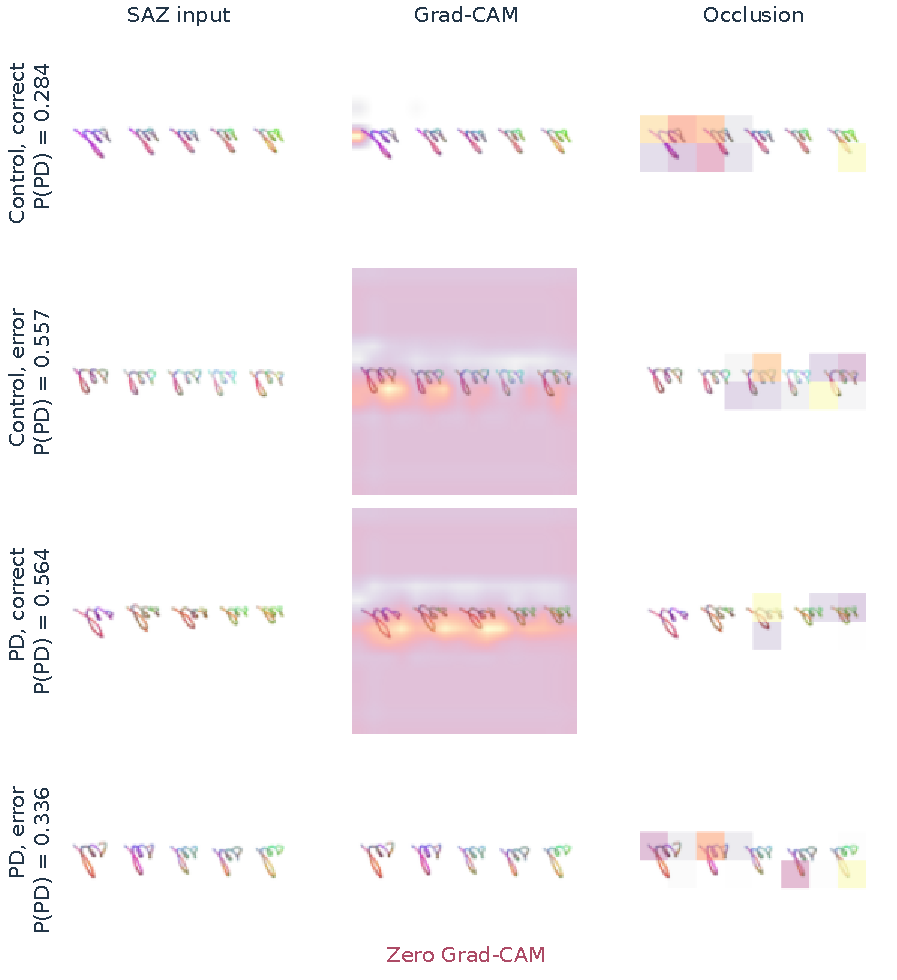
\includegraphics[width=0.72\textwidth]{xai_examples.pdf}
\caption{Task-4 explanations for correct and incorrect predictions from both classes. The four cases come from the first repetition, selected at median predicted-class confidence within each diagnosis/outcome stratum. Maps target the original predicted class and use its outer-test checkpoint. Opacity follows per-map attribution. The all-zero Grad-CAM in the PD error is retained. The CNN output is not a calibrated clinical probability.}
\label{fig:xai-examples}
\end{figure*}
\noindent
We apply XAI after freezing all outer checkpoints. Each image is explained by the exact checkpoint that produced its held-out prediction, rather than by a model fitted later to the entire cohort.

Grad-CAM weights convolutional activation maps with gradients of a target score \cite{Selvaraju2017}. We target the originally predicted class and use the last ReLU before the fourth pooling layer. At this point the spatial map is $16\times16$ for a $128\times128$ input. For activation map $A^k$ and predicted-class logit $g_c$, the attribution is
\begin{equation}
 L_c=\operatorname{ReLU}\!\left(\sum_k\alpha_k^c A^k\right),
 \quad \alpha_k^c=\frac{1}{UV}\sum_{u,v}\frac{\partial g_c}{\partial A^k_{uv}}.
\end{equation}
For the single output logit $g$, the PD target is $g_c=g$ and the H target is $g_c=-g$. The positive map is interpolated to input size and divided by its maximum when nonzero. Heatmap colours express attribution magnitude, independently of the input's semantic channels.

We calculate Grad-CAM for all 2,985 held-out predictions. A separate occlusion analysis replaces each non-overlapping $16\times16$ input patch with white and measures the decrease in confidence for the original predicted class. Negative changes are clipped to zero for the spatial occlusion map. This analysis covers all 597 predictions in the first repetition.

Figure~\ref{fig:xai-examples} illustrates correct and incorrect T4 predictions from both diagnosis classes, selected by the rule in its caption before inspecting the explanations. The aggregate analyses cover every task.

\subsection{Spatial Concentration and Perturbation}
\begin{figure*}[t]
\centering
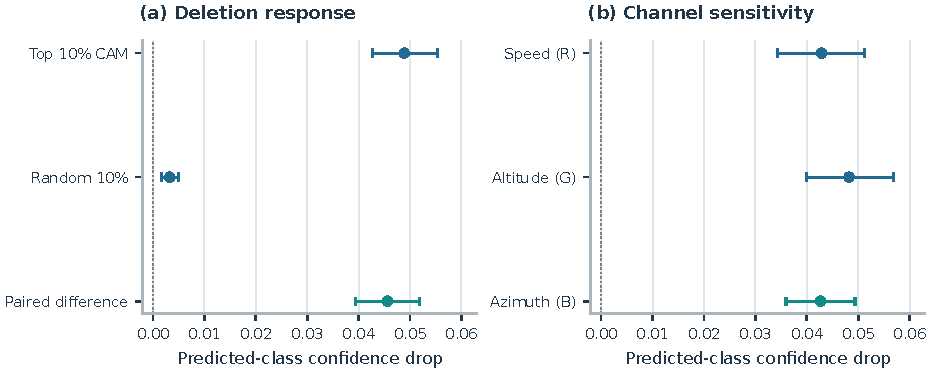
\includegraphics[width=\textwidth]{xai_validation.pdf}
\caption{Confidence changes for the originally predicted class. Left: deleting the top 10\% Grad-CAM pixels versus equal-area random deletion. Right: whitening each semantic channel. Intervals resample participants after averaging repeats and tasks. These perturbations measure sensitivity of the frozen CNN; the random control does not match foreground overlap, and channel removal also changes colour contrast.}
\label{fig:xai-validation}
\end{figure*}
\noindent
We define foreground as pixels with at least one channel below 250, matching the preprocessing. Foreground enrichment is the fraction of attribution inside that mask divided by the fraction of image area occupied by the mask. A uniform nonzero attribution map has enrichment one.

The participant-averaged Grad-CAM enrichment is 1.803, with interval [1.723, 1.884], indicating concentration around the rendered writing. There are 174 all-zero Grad-CAM maps, 5.83\% of the predictions. Enrichment is undefined for those maps, which are omitted before aggregation.

To test sensitivity to the highlighted pixels (Figure~\ref{fig:xai-validation}), we whiten the 10\% of input pixels with the greatest Grad-CAM values. Confidence in the original class falls by 0.0489 on average, with interval [0.0427, 0.0553]. An equal-area random deletion gives a drop of 0.0033 [0.0016, 0.0050]. The paired advantage of the directed deletion is 0.0456 [0.0395, 0.0518]. Before bootstrapping, repeated predictions are averaged within each participant and task, and tasks are averaged within participant.

Deletion summaries retain all 2,985 predictions, including the 174 all-zero maps. For those maps, the selected pixels follow the ranking routine's tie handling and carry no attribution-based preference.

The random control matches the number of replaced pixels but not their overlap with foreground or spatial shape. Whitening can also create inputs outside the training distribution. The deletion contrast therefore measures sensitivity under these perturbations and does not fully establish attribution faithfulness.

The two attribution methods show little spatial agreement. Median pixelwise Spearman correlation between Grad-CAM and occlusion is $-$0.0121 across 540 nonconstant pairs; the remaining 57 correlations are undefined. Concentration on handwriting therefore does not imply agreement about which regions influence the prediction.

We also reinitialize all network weights and compare Grad-CAM for one deterministically chosen held-out image per checkpoint. The 200 checks cover only 11 distinct participants because the selection rule repeatedly chooses the first identifier in each test partition. The median trained--random correlation is 0.0276 among 160 nonconstant pairs. Low agreement is consistent with dependence on learned weights, but the limited participant coverage and excluded constant maps constrain this check.

\subsection{Sensitivity to the Encoded Channels}
\noindent
Replacing a whole colour channel with white tests the CNN's sensitivity to that input component. Across the held-out predictions, the mean confidence drops are 0.0429 for speed, 0.0482 for altitude and 0.0427 for azimuth. Their intervals are [0.0343, 0.0512], [0.0400, 0.0568] and [0.0360, 0.0494], respectively.

These similar global values conceal task variation. Speed has the largest average effect on the spiral, while its effect on T6 is slightly negative. Removing a channel alters colour contrast as well as its coded measurement. The perturbation therefore cannot rank the underlying physiological signals or settle the speed-versus-pressure choice in the earlier SVM experiment.

These checks show sensitivity to writing regions and to all three input channels. They do not identify a disease-specific image feature.

\section{\uppercase{Discussion}}
\label{sec:discussion}

\noindent
The three experiments indicate that the classifiers use the pen dynamics encoded in the minimaps. When the static trace was available and favoured by ties, training-only selection chose a dynamic encoding in 24 of 25 training sets in Experiment~2, and in 23 of 25 with LPQ and 24 of 25 with ResNet18 in Experiment~3. Displacing the signals within strokes lowered recording-level macro F1, most under joint permutation, so the position of each value along the trajectory matters and not only the colours present. The benefit is clearest on the spiral, the drawing task, where $SAZ$ added 0.0802 in Experiment~1 and permutation removed 0.0609 in Experiment~2.

The gains depend on the task (Figure~\ref{fig:heatmap}). One encoding chosen for all eight tasks averages gains on the spiral and T6 with losses on T2, T3 and T5, which keeps its eight-task mean close to the static trace, whereas on the homogeneous letter patterns of T2--T4 the selected encoding gives the best participant-level decisions. Choosing encodings per task, rather than one for the whole protocol, is a direct way to exploit this dependence.

The pipelines are strong on different tasks (Table~\ref{tab:per-task}): minimaps with LPQ lead the spiral, kinematic attributes lead T2, T3 and the sentence, and minimaps with ResNet18 lead T4--T7 and the eight-task mean. The representation therefore works with both a handcrafted texture descriptor and pretrained convolutional features. The complementarity between the image and kinematic pipelines, each strongest on a different endpoint, motivates combining them. Shortening the protocol from eight tasks to three improved both the minimap LPQ and the kinematic pipelines, which reduces the number of exercises, although assessment time and clinical burden were not evaluated.

\section{\uppercase{Conclusion}}
\label{sec:conclusion}
\noindent
This initial study introduced pseudodynamic minimaps, a new image representation that places pen speed, pressure, altitude and azimuth as colour along the handwriting trajectory. Evaluated on PaHaW with participant-separated partitions, the representation was preferred over static traces by training-only selection, displacing the dynamics along each stroke lowered its performance, and on the three repeated-pattern tasks it gave the best participant-level decisions among the four compared pipelines. These results indicate that pseudodynamic minimaps are an effective way to bring pen dynamics into image-based handwriting analysis for Parkinson's disease.

The evidence comes from 75 participants of a single dataset that also informed the design of the experiments, so the size of the gains remains uncertain and independent cohorts are needed to confirm them. A source package with the code and configurations of all experiments supports that validation; the original recordings are not redistributed.

Future work will choose encodings per task, combine minimaps with kinematic descriptors, and fine-tune pretrained networks on the minimaps. A direct comparison with published PaHaW results is also left for future work. It requires more than citing reported accuracies: each method has to be re-implemented and evaluated under the same participant-separated partitions, without selecting tasks or features on test participants.

\bibliographystyle{apalike}
{\small\bibliography{refs}}
\end{document}
